\section{Подсчёт площадей многоугольников}

\paragraph{Основание и высота.}\label{1938/245}
Условимся одну из сторон треугольника или параллелограмма называть \rindex{основание}\textbf{основанием} этих многоугольников, а перпендикуляр, опущенный на эту сторону из вершины треугольника или из какой-нибудь точки противоположной стороны параллелограмма, будем называть \rindex{высота}\textbf{высотой}.

В прямоугольнике за высоту можно взять сторону, перпендикулярную к той, которая принята за основание.

В трапеции основаниями называют обе параллельные стороны, а высотой — общий перпендикуляр между ними.

Основание и высота прямоугольника называются его \rindex{измерения!прямоугольника}\textbf{измерениями}.

\paragraph{}\label{1938/246}
\so{Теорема}.
\textbf{\emph{Площадь прямоугольника равна произведению его основания на высоту.}}

При доказательстве могут представиться три случая:


1) Длины основания и высоты (измеренных одной и той же единицей) выражаются \so{целыми числами}.

\begin{wrapfigure}{o}{29mm}
\vskip-4mm
\centering
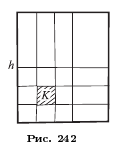
\includegraphics{mppics/ris-242}
\caption{}\label{1938/ris-242}
\end{wrapfigure}

Пусть у данного прямоугольника (рис.~\ref{1938/ris-242}) основание равно целому числу $b$ линейных единиц, а высота — целому числу $h$ тех же единиц.
Разделим основание на $b$ и высоту на $h$ равных частей, проведём через точки деления ряд прямых, параллельных высоте, и другой ряд прямых, параллельных основанию.
От взаимного пересечения этих прямых образуются некоторые четырёхугольники.

Возьмём какой-нибудь один из них, например четырёхугольник $K$ (покрытый на рисунке штрихами).
Так как стороны этого четырёхугольника, по построению, параллельны соответствующим сторонам данного прямоугольника, то все углы его прямые;
значит, четырёхугольник $K$ есть прямоугольник.
С другой стороны, каждая сторона этого прямоугольника равна расстоянию между соседними параллельными прямыми, то есть равна одной и той же линейной единице. 
Значит, прямоугольник $K$ представляет собой квадрат, а именно, ту квадратную единицу, которая соответствует взятой линейной единице (если, например, за линейную единицу принят линейный сантиметр, то площадь квадрата $K$ есть квадратный сантиметр).

Так как сказанное об одном четырёхугольнике справедливо и для всякого другого, то, значит, проведением указанных параллельных прямых мы разбиваем всю площадь данного прямоугольника на квадратные единицы.
Найдём их число.

Очевидно, что ряд прямых, параллельных основанию, разделяет прямоугольник на столько равных горизонтальных полос, сколько в высоте содержится линейных единиц, то есть на $h$ равных полос.
С другой стороны, ряд прямых, параллельных высоте, разбивает каждую горизонтальную полосу на столько квадратных единиц, сколько в основании содержится линейных единиц, то есть на $b$ квадратных единиц.
Значит, всех квадратных единиц окажется $b\cdot h$.
Таким образом.
\[\text{площадь прямоугольника} = b\cdot h.\]
то есть она равна произведению основания на высоту.

2) Длины основания и высоты (измеренных одной и той же единицей) выражаются \so{дробными числами}.

Пусть, например, у данного прямоугольника
\[\text{основание} = 3\tfrac12=\tfrac72~\text{линейных единиц.}\]
\[\text{высота} = 4\tfrac35 = \tfrac{23}5~\text{той же единицы.}\]
Приведя дроби к одинаковому знаменателю, получим:
\[\text{основание} = \tfrac{35}{10};
\quad
\text{высота} = \tfrac{46}{10}.
\]
Примем $\tfrac1{10}$ долю линейной единицы за новую единицу длины.

Тогда мы можем сказать, что основание содержит 35 этих новых единиц, а высота 46 тех же единиц.
Значит, по доказанному, в случае 1-м, площадь прямоугольника равна $35 \cdot 46$ таких квадратных единиц, которые соответствуют $\tfrac1{100}$ новой единице длины.
Но эта квадратная единица составляет часть квадратной единицы, соответствующей прежней линейной единице;
значит, площадь прямоугольника в прежних квадратных единицах равна:
\[\frac{35\cdot 46}{100}=\frac{35}{10}\cdot\frac{46}{10}=3\tfrac12\cdot4\tfrac35(\text{квадратных единиц}).\]

3) Основание и высота (или только одно из этих измерений) несоизмеримы с единицей длины, и, следовательно, их длины выражаются \so{иррациональными числами}.

В этом случае можно довольствоваться приближённым результатом измерения площади с желаемой степенью точности.
Но можно и в этом случае найти точную меру площади прямоугольника.

\begin{wrapfigure}{O}{45mm}
\centering
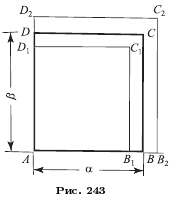
\includegraphics{mppics/ris-243}
\caption{}\label{1938/ris-243}
\end{wrapfigure}

Пусть длина основания $AB$ прямоугольника $ABCD$ (рис.~\ref{1938/ris-243}) выражается  числом $\alpha$, а для высоты $AD$ — числом $\beta$.
Каждое из этих чисел может быть представлено в виде бесконечной десятичной дроби (§~\ref{1938/150}).
Возьмём приближённые значения этих чисел в виде десятичных дробей с $n$ десятичными знаками сначала с недостатком, затем с избытком.
Приближённые значения с недостатком обозначим через $\alpha_n$ (для первого числа) и $\beta_n$ (для второго числа), а приближённые значения с избытком соответственно через  $\alpha_n'$ и $\beta_n'$.

Отложим на основании $AB$ от точки $A$ сначала отрезок $AB_1$ длины $\alpha_n$, затем отрезок $AB_2$ длинны  $\alpha_n'$.
Очевидно, 
\[AB_1\le AB\le AB_2.\]
Отложим, далее, на высоте $AD$ от точки $A$ отрезки $AD_1$ и $AD_2$, длины которых равны соответственно $\beta_n$ и $\beta_n'$.
Очевидно, 
\[AD_1\le AD\le AD_2.\]

Построим вспомогательные прямоугольники $AB_1C_1D_1$ и $AB_2C_2D_2$, у каждого из них основание и высота выражаются рациональными числами:
\begin{align*}
AB_1&=\alpha_n,
&
AD_1&=\beta_n,
\\
AB_2&=\alpha_n',
&
AD_2&=\beta_n'.
\end{align*}
Поэтому, согласно доказанному в случае 2-м.
\begin{align*}
\text{площадь}~AB_1C_1D_1 &= \alpha_n\cdot \beta_n, 
\\
\text{площадь}~AB_2C_2D_2 &= \alpha_n'\cdot \beta_n'. 
\end{align*}

Поскольку прямоугольник $AB_1C_1D_1$ составляет часть прямоугольника $ABCD$, 
а прямоугольник $ABCD$ составляет часть прямоугольника $AB_2C_2D_2$;
имеем
\[\alpha_n\cdot \beta_n\le\text{площадь}~ABCD\le\alpha_n'\cdot \beta_n'.\]
Это двойное неравенство остаётся верным при всяком значении $n$, то есть оно остаётся верным, с какой бы точностью мы ни находили приближённые значения чисел $\alpha$ и $\beta$.
Значит, мы можем сказать, что площадь $ABCD$ должна выражаться таким числом, которое больше произведения любых приближённых значений чисел $\alpha$ и $\beta$, если эти значения взяты с недостатком, но меньше произведения любых их приближённых значений, если эти значения взяты с избытком.
Но существует единственное такое число, это произведение чисел $\alpha$ и $\beta$ (§~\ref{1938/154}).
Следовательно 
\[\text{площадь}~ABCD=\alpha\cdot \beta.\]
Таким образом, и в этом случае площадь прямоугольника равна произведению основания на высоту.

\paragraph{}\label{1938/247}
\so{Теорема}.
\textbf{\emph{Площадь параллелограмма}} ($ABCD$, рис.~\ref{1938/ris-244} и \ref{1938/ris-245}) \textbf{\emph{равна произведению основания на высоту.}}

На основании $AD$ (на том и другом рисунке) построим прямоугольник $AEFD$, у которого сторона $EF$ составляет продолжение стороны $BC$.

При этом могут представиться два случая:

\begin{figure}[h]
\begin{minipage}{.58\textwidth}
\centering
\includegraphics{mppics/ris-244}
\end{minipage}
\hfill
\begin{minipage}{.38\textwidth}
\centering
\includegraphics{mppics/ris-245}
\end{minipage}

\medskip

\begin{minipage}{.58\textwidth}
\centering
\caption{}\label{1938/ris-244}
\end{minipage}
\hfill
\begin{minipage}{.38\textwidth}
\centering
\caption{}\label{1938/ris-245}
\end{minipage}
\vskip-4mm
\end{figure}

1) сторона $BC$ лежит вне стороны $EF$ и 2) сторона $BC$ частью совпадает с $EF$ (первый случай изображён на рис.~\ref{1938/ris-244}, второй — на рис.~\ref{1938/ris-245}).
Докажем, что и в том, и другом случае
\[\text{площадь}~ABCD = \text{площади}~AEFD.\]
Если параллелограмм дополним треугольником $AEB$, а прямоугольник дополним треугольником $DFC$, то мы получим одну и ту же трапецию $AECD$.
Так как дополняющие треугольники равны (они имеют по две стороны и углу, заключённому между ними, соответственно равными), то параллелограмм и прямоугольник должны быть равновелики.
Но площадь $AEFD=b\cdot h$;
следовательно, и площадь $ABCD=b\cdot h$, причём $b$ можно рассматривать как основание параллелограмма и $h$ — как его высоту.

%309(1914) замечание о равносоставленности

\paragraph{}\label{1938/248}
\so{Теорема}.
\textbf{\emph{Площадь треугольника}} ($ABC$, рис.~\ref{1938/ris-246}) \textbf{\emph{равна половине произведения основания на высоту.}}

Проведём $BE \parallel  AC$ и $AE \parallel BC$.
Тогда получим параллелограмм $AEBC$, площадь которого, по доказанному, равна $b\cdot h$.
Поскольку треугольники $ABC$ и $BAE$ равны, площадь $\triangle ABC$ составляет половину площади $ADBC$;
то есть
\[\text{площадь}~ \triangle ABC=\tfrac12b\cdot h.\]

\begin{figure}[h]
\begin{minipage}{.48\textwidth}
\centering
\includegraphics{mppics/ris-246}
\end{minipage}
\hfill
\begin{minipage}{.48\textwidth}
\centering
\includegraphics{mppics/ris-247}
\end{minipage}

\medskip

\begin{minipage}{.48\textwidth}
\centering
\caption{}\label{1938/ris-246}
\end{minipage}
\hfill
\begin{minipage}{.48\textwidth}
\centering
\caption{}\label{1938/ris-247}
\end{minipage}
\vskip-4mm
\end{figure}

\smallskip
\mbox{\so{Замечание}.}
Легко убедиться, что всякий треугольник разлагается на части, перемещением которых можно образовать прямоугольник, имеющий одинаковое с треугольником основание и высоту, вдвое меньшую высоты треугольника (рис.~\ref{1938/ris-247}).

\paragraph{}\label{1938/249}
\so{Следствия}.
1) \emph{Треугольники с равными основаниями и равными высотами равновелики.}

Если, например, вершину $B$ треугольника $ABC$ (рис.~\ref{1938/ris-248}) будем перемещать по прямой, параллельной основанию $AC$, а основание оставим то же самое, то площадь треугольника не будет изменяться.

\begin{figure}[h]
\begin{minipage}{.48\textwidth}
\centering
\includegraphics{mppics/ris-248}
\end{minipage}
\hfill
\begin{minipage}{.48\textwidth}
\centering
\includegraphics{mppics/ris-249}
\end{minipage}

\medskip

\begin{minipage}{.48\textwidth}
\centering
\caption{}\label{1938/ris-248}
\end{minipage}
\hfill
\begin{minipage}{.48\textwidth}
\centering
\caption{}\label{1938/ris-249}
\end{minipage}
\vskip-4mm
\end{figure}


2) \emph{Площадь прямоугольного треугольника равна половине произведения его катетов,} потому что один катет можно взять за основание, а другой — за высоту.

%+чертёж и замечания из 311(1914)

3) \emph{Площадь ромба равна половине произведения его диагоналей.}
Действительно, если $ABCD$ (рис.~\ref{1938/ris-249}) есть ромб, то его диагонали взаимно перпендикулярны.
Поэтому

\begin{center}
\begin{tabular}{rrcl}
 &$\text{площадь}~\triangle ABC$
 &$=$ 
 &$\tfrac12AC\cdot  OB$
\\
\raisebox{3mm}[3mm][3mm]{$+$} 
& 
$\text{площадь}~\triangle ACD$
&$=$ &$\tfrac12AC\cdot  OD$
\\
\hline
&$\text{площадь}~ABCD$ & $=$&$\tfrac12AC\cdot (OB+OD)=\tfrac12AC\cdot BD.$
\end{tabular}
\end{center}

4) \emph{Площади двух треугольников относятся как произведения их оснований на высоты} (множитель $\tfrac12$ сокращается).


\paragraph{}\label{1938/250}
\so{Теорема}.
\textbf{\emph{Площадь трапеции равна произведению полусуммы оснований на высоту.}}

Проведя в трапеции $ABCD$ (рис.~\ref{1938/ris-250}) диагональ $AC$, мы можем рассматривать её площадь как сумму площадей двух треугольников $CAD$ и $ABC$.
Поэтому
\[\text{площадь трапеции}~ABCD
=\tfrac12AD\cdot  h+\tfrac12BC\cdot  h= 
\tfrac12(AD+BC) \cdot  h.\]

\begin{figure}[h]
\begin{minipage}{.48\textwidth}
\centering
\includegraphics{mppics/ris-250}
\end{minipage}
\hfill
\begin{minipage}{.48\textwidth}
\centering
\includegraphics{mppics/ris-251}
\end{minipage}

\medskip

\begin{minipage}{.48\textwidth}
\centering
\caption{}\label{1938/ris-250}
\end{minipage}
\hfill
\begin{minipage}{.48\textwidth}
\centering
\caption{}\label{1938/ris-251}
\end{minipage}
\vskip-4mm
\end{figure}

\paragraph{}\label{1938/251}
\so{Следствие}.
Если $MN$ (рис.~\ref{1938/ris-251}) есть средняя линия трапеции, то, как известно (§~\ref{1938/99}).
\[MN = \tfrac12(AD+BC).\]
Поэтому
\[\text{площадь трапеции}~ABCD=MN\cdot  h.\]
то есть \emph{площадь трапеции равна произведению средней линии на высоту.}
Это же можно видеть и непосредственно из рис.~\ref{1938/ris-251}.

\paragraph{}\label{1938/252}
\so{Теорема}.
\textbf{\emph{Площадь всякого описанного многоугольника равна произведению периметра на половину радиуса.}}

\begin{wrapfigure}{o}{35mm}
\centering
\includegraphics{mppics/ris-252}
\caption{}\label{1938/ris-252}
\end{wrapfigure}

Соединив центр $O$ (рис.~\ref{1938/ris-252}) со всеми вершинами описанного многоугольника, мы разделим его на треугольники, в которых за основания можно взять стороны многоугольника, а за высоты — радиус круга.

Обозначив этот радиус через $R$, будем иметь:
\begin{align*}
\text{площадь}~\triangle AOB&=AB \cdot  \tfrac12R,
\\
\text{площадь}~\triangle BOC &= BC \cdot  \tfrac12R\quad\text{и~т.~д.}
\end{align*}
Следовательно,
\[\text{площадь}~ABCDE = (AB+BC+CD+DE+EA) \cdot  \tfrac12R= P \cdot \tfrac12R,\]
где буквой $P$ обозначен периметр многоугольника.

\smallskip
\so{Следствие}.
\emph{Площадь правильного многоугольника равна произведению периметра на половину апофемы,} потому что всякий правильный многоугольник можно рассматривать как описанный около круга, у которого радиус есть апофема.

\paragraph{Площадь неправильного многоугольника.}\label{1938/253}
Для нахождения площади какого-нибудь неправильного многоугольника можно его разбить на треугольники (например, диагоналями), вычислить площадь каждого треугольника в отдельности и результаты сложить.

{\sloppy

\paragraph{}\label{1938/254}
\mbox{\so{Задача}.}
\emph{Построить треугольник, равновеликий данному многоугольнику} ($ABCDE$, рис.~\ref{1938/ris-253}).

}

\begin{wrapfigure}{o}{38mm}
\vskip-2mm
\centering
\includegraphics{mppics/ris-253}
\caption{}\label{1938/ris-253}
\end{wrapfigure}

Какой-нибудь диагональю $AC$ отсекаем от данного многоугольника треугольник $ABC$.
Через ту вершину $B$ этого треугольника, которая лежит против взятой диагонали, проводим прямую $MN\parallel AC$.
Затем продолжим одну из сторон $EA$ или $DC$, прилежащих к отсечённому треугольнику, до пересечения с прямой $MN$ (на рисунке продолжена сторона $EA$).
Точку пересечения $F$ соединим прямой с $C$.
Треугольники $CBA$ и $CFA$ равновелики, так как у них общее основание $AC$, а вершины $B$ и $F$ лежат на прямой, параллельной основанию.

Если от данного многоугольника отделим $\triangle CBA$ и вместо него приложим равновеликий ему $\triangle CFA$, то величина площади не изменится;
следовательно, данный многоугольник равновелик многоугольнику $FCDE$, у которого, очевидно, число углов на единицу меньше, чем у данного многоугольника.

Таким же приёмом можно число углов полученного многоугольника уменьшить ещё на единицу и продолжать такое последовательное уменьшение до тех пор, пока не получится треугольник ($FCG$ на нашем рисунке).

\paragraph{}\label{1938/255}
\so{Задача}.
\emph{Построить квадрат, равновеликий данному многоугольнику.}

Сначала преобразовывают многоугольник в равновеликий треугольник, а затем этот треугольник — в квадрат.
Пусть основание и высота треугольника $b$ и $h$, а сторона искомого квадрата $x$.
Тогда площадь первого равна $b\cdot h$, а второго — $x^2$; 
следовательно,
\begin{align*}
\tfrac12 b\cdot h&=x^2,
\end{align*}
откуда
$\frac12 b:{x}=x:h$,
то есть $x$ есть средняя пропорциональная между $\tfrac12 b$ и $h$.
Значит, сторону квадрата можно построить способом, указанным раньше (§~\ref{1938/190}) для нахождения средней пропорциональной.

{\sloppy

\smallskip
\so{Замечание}.
Преобразование данного многоугольника в треугольник не всегда необходимо.
Например, если речь идёт о преобразовании в квадрат данной трапеции, то достаточно найти среднюю пропорциональную между высотой трапеции и её средней линией и на полученном отрезке построить квадрат.

}

\paragraph{}\label{1938/256}
\so{Задача}.
\emph{Вычислить площадь $S$ треугольника, зная длины $a$, $b$ и $c$ его сторон.}

\begin{wrapfigure}{o}{40mm}
\centering
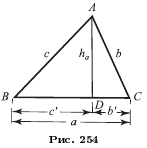
\includegraphics{mppics/ris-254}
\caption{}\label{1938/ris-254}
\end{wrapfigure}

Пусть высота $\triangle ABC$ (рис.~\ref{1938/ris-254}), опущенная на сторону $a$, есть $h_a$.
Тогда
\[S=\tfrac12ah_a.\]

Чтобы найти высоту $h_a$, возьмём равенство (§~\ref{1938/194}):
\[b^2 =  a^2+c^2 -2ac'\]
и определим из него отрезок $c'$.
\[c'=\frac{a^2+c^2-b^2}{2a}.\]

Из $\triangle ABD$ находим:
\begin{align*}
h_a&=\sqrt{c^2-(c')^2}=
\\
&=\sqrt{c^2-\left(\frac{a^2+c^2-b^2}{2a}\right)^2}=
\\
&=\frac{1}{2a}\sqrt{4a^2c^2-(a^2+c^2-b^2)^2}.
\end{align*}
Преобразуем подкоренное выражение так:
\begin{align*}
4a^2c^2&-(a^2+c^2-b^2)^2=
\\
&=[2ac+(a^2+c^2-b^2)]\cdot[2ac-(a^2+c^2-b^2)]=
\\
&=[(a^2+2ac+c^2)-b^2]\cdot[b^2-(a^2-2ac+c^2)]=
\\
&=[(a+c)^2-b^2]\cdot[b^2-(a-c)^2]=
\\
&=(a+c+b)(a+c-b)(b+a-c)(b-a+c).
\end{align*}
Следовательно,
\[S=\tfrac12 ah_a=\tfrac14\sqrt{(a+c+b)(a+c-b)(b+a-c)(b-a+c)}.\]
(Так как в треугольнике сумма любых двух сторон больше третьей, то все разности $a+b-c$, $a+c-b$ и $b+c-a$ — числа положительные.)

Если положим, что $a+b+c=2p$, то
\[a+c-b=(a+b+c)-2b=2p-2b=2(p-b).\]
Подобно этому
\begin{align*}
 b+a-c&=2(p-c);
 \\
 b+c-a&=2(p-a).
\end{align*}
Тогда
\begin{align*}
S&=\tfrac14\sqrt{2p\cdot2(p-a)\cdot2(p-b)\cdot2(p-c)},
\intertext{то есть}
S&=\sqrt{p(p-a)(p-b)(p-c)}.
\end{align*}
Это выражение известно под названием \rindex{формула Герона}\textbf{формулы Герона} (по имени математика Герона из Александрии, жившего приблизительно в III—II веках до нашей эры).

\smallskip
\so{Частный случай.}
Площадь равностороннего треугольника со стороной $a$ выражается следующей формулой:
\begin{align*}S&=\sqrt{\frac{3a}2\cdot \frac a2\cdot \frac a2\cdot \frac a2}=
 \\
 &=\frac{a^2\sqrt{3}}{4}.
\end{align*}


\subsection*{Теорема Пифагора и основанные на ней задачи}

\paragraph{}\label{1938/257}
\so{Теорема}.
\textbf{\emph{Сумма площадей квадратов, построенных на катетах прямоугольного треугольника, равна площади квадрата, построенного на гипотенузе этого треугольника.}}

Это предложение является другой формой теоремы Пифагора, доказанной ранее (§~\ref{1938/191}):
квадрат числа, измеряющего длину гипотенузы, равен сумме квадратов чисел, измеряющих длины катетов.
Действительно, квадрат числа, измеряющего длину отрезка, и является мерой площади квадрата, построенного на этом отрезке.
Поэтому теорема §~\ref{1938/191} равносильна указанной теореме Пифагора.

Приведём другое доказательство теоремы Пифагора, основанное не на вычислении площадей, а на непосредственном их сравнении между собой.

\smallskip
\mbox{\so{Доказательство}} (Евклида).
Пусть $ABC$ (рис.~\ref{1938/ris-255}) — прямоугольный треугольник, а $BDEA$, $AFGC$ и $BCKH$ — квадраты, построенные на его катетах и гипотенузе;
требуется доказать, что сумма площадей двух первых квадратов равна площади третьего квадрата.

Проведём $AM\perp BC$.
Тогда квадрат $BCKH$ разделится на два прямоугольника.
Докажем, что прямоугольник $BLMH$ равновелик квадрату $BDEA$, а прямоугольник $LCKM$ равновелик квадрату $AFGC$.

\begin{wrapfigure}{o}{47mm}
\centering
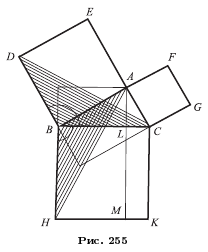
\includegraphics{mppics/ris-255}
\caption{}\label{1938/ris-255}
\end{wrapfigure}

Проведём вспомогательные прямые $DC$ и $AH$.
Рассмотрим два треугольника, покрытые на рисунке штрихами.
Треугольник $BCD$, имеющий основание $BD$, общее с квадратом $BDEA$, а высоту $CN$, 
равную высоте $AB$ этого квадрата, равновелик половине квадрата.
Треугольник $ABH$, имеющий основание $BH$, общее с прямоугольником $BLMH$, и высоту $AP$, 
равную высоте $BL$ этого прямоугольника, равновелик половине его.
Сравнивая эти два треугольника между собой, находим, что у них $BD = BA$ и $BC=BH$ (как стороны квадрата);
сверх того $\angle DBC=\angle ABH$, так как каждый из этих углов состоит из общей части $ABC$ и прямого угла.
Значит, треугольники $ABH$ и $DBC$ равны.
Отсюда следует, что прямоугольник $BLMH$ равновелик квадрату $BDEA$.

Соединив $G$ с $B$ и $A$ с $K$, мы совершенно так же докажем, что прямоугольник $LCKM$ равновелик квадрату $AFGC$.
Отсюда следует, что квадрат $BCKH$ равновелик сумме квадратов $BDEA$ и $AFGC$.

%второе доказательство 321(1914)

\paragraph{}\label{1938/258}
\so{Задачи}.
1) \emph{Построить квадрат, площадь которого равна сумме площадей двух данных квадратов.}

Строим прямоугольный треугольник, у которого катетами были бы стороны данных квадратов.
Квадрат, построенный на гипотенузе этого треугольника, имеет площадь, равную сумме площадей данных квадратов.

2) \emph{Построить квадрат, площадь которого равна разности площадей двух данных квадратов.}

{

\begin{wrapfigure}{o}{50mm}
\vskip-0mm
\centering
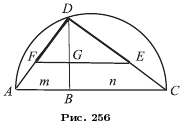
\includegraphics{mppics/ris-256}
\caption{}\label{1938/ris-256}
\end{wrapfigure}

Строим прямоугольный треугольник, у которого гипотенузой была бы сторона большего из данных квадратов, а катетом — сторона меньшего квадрата.
Квадрат, построенный на другом катете этого треугольника, является искомым.

3) \emph{Построить квадрат, площадь которого относится к площади данного квадрата как $m:n$.}

}

На произвольной прямой (рис. \ref{1938/ris-256}) откладываем отрезки $AB=m$ и $BC\z=n$, и на $AC$ как на диаметре описываем полуокружность.
Из точки $B$ восстанавливаем перпендикуляр $BD$ до пересечения с окружностью.
Проведя хорды $AD$ и $DC$, получим прямоугольный треугольник, у которого (§~\ref{1938/192})
\[\frac{AD^2}{DC^2}=\frac{AB}{BC}=\frac mn.\]
На катете $DC$ этого треугольника отложим отрезок $DF$, равный стороне данного квадрата,% 
\footnote{Если сторона данного квадрата больше $DC$, то точки $E$ и $E$ будут лежать на продолжениях катетов $DC$ и $DA$.}
и проведём $EF\parallel CA$.
Отрезок $DE$ есть сторона искомого квадрата, потому что
\[
\frac{DF}{DE}=\frac{AD}{DC},\]
откуда
\[\left(\frac{DF}{DE}\right)^2=\left(\frac{AD}{DC}\right)^2;\]
следовательно,
\[\frac{DF^2}{DE^2}=\frac{AD^2}{DC^2}=\frac mn.\]

\subsection*{Отношение площадей подобных многоугольников}

\paragraph{}\label{1938/259}
\so{Теорема}.
\textbf{\emph{Площади двух треугольников, имеющих по равному углу, относятся как произведения сторон, заключающих эти углы.}}

Пусть в треугольниках $ABC$ и $A_1B_1C_1$ (рис.~\ref{1938/ris-257}) углы $A$ и $A_1$ равны.

\begin{figure}[h]
\centering
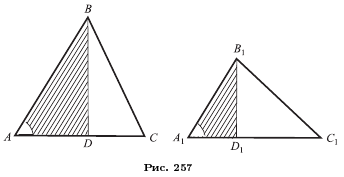
\includegraphics{mppics/ris-257}
\caption{}\label{1938/ris-257}
\end{figure}

Проведя высоты $BD$ и $B_1D_1$, будем иметь:
\[\frac{\text{площадь}~ABC}{\text{площадь}~A_1B_1C_1}=\frac{AC\cdot  BD}{A_1C_1\cdot  B_1D_1}=\frac{AC}{A_1C_1}\cdot\frac{BD}{B_1D_1}.\]
Треугольники $ABD$ и $A_1B_1D_1$ подобны ($\angle A = \angle A_1$ и $\angle D\z=\angle D_1$), поэтому 
\[\frac{BD}{B_1D_1}=\frac{AB}{A_1B_1};\]
заменив первое отношение вторым, получим:
\[\frac{\text{площадь}~ABC}{\text{площадь}~A_1B_1C_1}=\frac{AC}{A_1C_1}\cdot\frac{BD}{B_1D_1}=\frac{AC}{A_1C_1}\cdot\frac{AB}{A_1B_1}.\]

{\sloppy

\paragraph{}\label{1938/260}
\so{Теорема}.
\textbf{\emph{Площади подобных треугольников или многоугольников относятся как квадраты соответственных сторон.}}

}

1) Если $ABC$ и $A_1B_1C_1$ — два подобных треугольника, то углы одного равны соответственно углам другого;
пусть $\angle A \z= \angle A_1$, $\angle B\z=\angle B_1$ и $\angle C = \angle C_1$.
Применим к ним предыдущую теорему:
\[\frac{\text{площадь}~ABC}{\text{площадь}~A_1B_1C_1}=
 \frac{AB\cdot  AC}{A_1B_1\cdot  A_1C_1}=
 \frac{AB}{A_1B_1}\cdot
 \frac{AC}{A_1C_1}.
 \eqno(1)
\]
Но из подобия треугольников следует:
\[\frac{AB}{A_1B_1}=\frac{AC}{A_1C_1}=\frac{BC}{B_1C_1} \eqno(2)\]
Поэтому в равенстве (1) мы можем каждое из отношений $\frac{AB}{A_1B_1}$ и $\frac{AC}{A_1C_1}$ заменить любым отношением ряда (2);
следовательно:
\begin{align*}
\frac{\text{площадь}~ABC}{\text{площадь}~A_1B_1C_1}&=
\left(\frac{AB}{A_1B_1}\right)^2=
\left(\frac{AC}{A_1C_1}\right)^2=
\left(\frac{BC}{B_1C_1}\right)^2=
\\
&=\frac{AB^2}{A_1B_1^2}=
\frac{AC^2}{A_1C_1^2}=
\frac{BC^2}{B_1C_1^2}.
\end{align*}

2) Если $ABCDE$ и $A_1B_1C_1D_1E_1$ (рис.~\ref{1938/ris-258}) — два подобных многоугольника, то их можно, как мы видели (§~\ref{1938/171}), разложить на одинаковое число подобных и одинаково расположенных треугольников.

\begin{figure}[h]
\centering
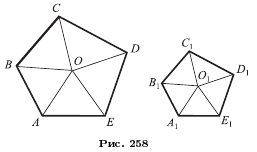
\includegraphics{mppics/ris-258}
\caption{}\label{1938/ris-258}
\end{figure}

Пусть эти треугольники будут:
$AOB$ и $A_1O_1B_1$, $BOC$ и $B_1O_1C_1$ и~т.~д.
Согласно доказанному в первой части этой теоремы, мы получим пропорции:
\begin{align*}
\frac{\text{площадь}~AOB}{\text{площадь}~A_1O_1B_1}&=\left(\frac{AB}{A_1B_1}\right)^2;
\\
\frac{\text{площадь}~BOC}{\text{площадь}~B_1O_1C_1}&=\left(\frac{BC}{B_1C_1}\right)^2\quad\text{и так далее}
\end{align*}
Но из подобия многоугольников следует:
\[\frac{AB}{A_1B_1}=\frac{BC}{B_1C_1}=\frac{CD}{C_1D_1}=\dots\]
и потому
\[\left(\frac{AB}{A_1B_1}\right)^2=\left(\frac{BC}{B_1C_1}\right)^2=\left(\frac{CD}{C_1D_1}\right)^2=\dots\]

Значит,
\begin{align*}
\frac{\text{площадь}~AOB}{\text{площадь}~A_1O_1B_1}
&=
\frac{\text{площадь}~BOC}{\text{площадь}~B_1O_1C_1}
=
\\
&=
\frac{\text{площадь}~COD}{\text{площадь}~C_1O_1D_1}=
\\
&=\dots,
\end{align*}
откуда
\begin{align*}
&\frac{\text{площадь}~AOB+\text{площадь}~BOC+\dots+\text{площадь}~EOA}{\text{площадь}\,A_1O_1B_1+\text{площадь}\,B_1O_1C_1+\dots+\text{площадь}\,E_1O_1A_1}
=
\\
&\quad=
\frac{\text{площадь}~ABCDE}{\text{площадь}~A_1B_1C_1D_1E_1}
=\frac{AB^2}{A_1B_1^2}.
\end{align*}

\smallskip
\so{Следствие}.
\emph{Площади правильных  $n$-угольников относятся как квадраты сторон, или квадраты радиусов описанных окружностей, или квадраты апофем.}

\begin{wrapfigure}[7]{r}{47mm}
\vskip-6mm
\centering
\includegraphics{mppics/ris-extra-9}
\caption{}\label{extra/ris-9}
\end{wrapfigure}

\paragraph{}\label{extra/pifagor} Покажем, что теорему Пифагора (§~\ref{1938/191}) можно получить как следствие из теоремы в §~\ref{1938/260}. 

Пусть $ABC$ (рис.~\ref{extra/ris-9}) есть прямоугольный треугольник, $AD$ — перпендикуляр, опущенный на гипотенузу из вершины прямого угла.
Треугольники $ABC$, $DBA$ подобны, так как имеют по прямому углу и ещё общий угол $B$.
Значит 
\[\frac{\text{площадь}~DBA}{\text{площадь}~ABC}=
 \frac{c^2}{a^2}.
\]

Точно также получаем, что
\[\frac{\text{площадь}~DAC}{\text{площадь}~ABC}=
 \frac{b^2}{a^2}.
\]

Поскольку треугольники $DBA$ и $DAC$ вместе составляют $\triangle ABC$, сумма площадей
$\triangle DBA$ и $\triangle DAC$ равна площади $\triangle ABC$.
Отсюда
\[\frac{b^2+c^2}{a^2}=1\]
или 
\[b^2+c^2=a^2.\]





\paragraph{}\label{1938/261}
\so{Задача}.
\emph{Разделить данный треугольник на $m$ равновеликих частей прямыми, параллельными его стороне.}

Пусть, например, требуется разделить $\triangle ABC$ (рис.~\ref{1938/ris-259}) на три равновеликие части отрезками, параллельными основанию $AC$.

Предположим, что искомые отрезки будут $DE$ и $FG$.
Очевидно, что если мы найдём отрезки $BE$ и $BG$, то определятся и отрезки $DE$ и $FG$.
Треугольники $BDE$, $BFG$ и $BAC$ подобны;
поэтому
\begin{align*}
\frac{\text{площадь}~BDE}{\text{площадь}~BAC}&=\frac{BE^2}{BC^2}
&&\text{и}
&\frac{\text{площадь}~BFG}{\text{площадь}~BAC}&=\frac{BG^2}{BC^2}.
\intertext{Но}
\frac{\text{площадь}~BDE}{\text{площадь}~BAC}&=\frac{1}{3}
&&\text{и}
&\frac{\text{площадь}~BFG}{\text{площадь}~BAC}&=\frac{2}{3}.
\intertext{Следовательно,}
\frac{BE^2}{BC^2}&=\frac13
&&\text{и}
&\frac{BG^2}{BC^2}&=\frac23,
\end{align*}
откуда
\begin{align*}
BE&=\sqrt{\tfrac13BC^2}=\sqrt{\tfrac13BC\cdot BC}
\intertext{и}
BG&=\sqrt{\tfrac23BC^2}=\sqrt{\tfrac23BC\cdot BC}
\end{align*}
Из этих выражений видим, что $BE$ есть средняя пропорциональная между $BC$ и $\tfrac13BC$, а $BG$ есть средняя пропорциональная между $BC$ и $\tfrac23BC$.

\begin{wrapfigure}{o}{45mm}
\centering
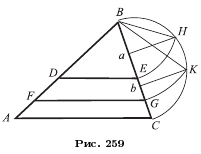
\includegraphics{mppics/ris-259}
\caption{}\label{1938/ris-259}
\end{wrapfigure}

Поэтому построение можно выполнить так:
разделим $BC$ на три равные части в точках $a$ и $b$;
опишем на $BC$ полуокружность;
из $a$ и $b$ восстановим к $BC$ перпендикуляры $aH$ и $bK$.
Хорды $HB$ и $KB$ будут искомыми средними пропорциональными;
первая — между всем диаметром $BC$ и его третьей частью $Ba$, вторая — между $BC$ и В$b$, то есть между $BC$ и $\tfrac23BC$.
Остаётся отложить эти хорды на $BC$ от точки $B$, тогда получим искомые точки $E$ и~$G$.

Подобным образом можно разделить треугольник на какое угодно число равновеликих частей.
